\section{Circuit Design}
\subsection{Low Noise Amplifier}
Low noise amplifiers(LNA) are typically one of the starting blocks in the front end receiver chain. LNAs need to exhibit low noise, high gain, and low power dissipation. The linearity doesn't need to be so good, but it can't be so bad as to limit the overall linearity of the chain. The noise figure needs to be low because the noise figure of the system can be approximately equal to the noise figure of the first block, assuming there is no other block in the system that isn't so large that it won't be scaled by the gain of the prior blocks. 

\subsubsection{Design Procedure}
As shown in Figure ~\ref{fig:lna}, there are two structures that are popularly used when designing LNAs:  cascode~\cite{Razavi} and current reuse~\cite{lna}. 

\begin{figure}[h]
   \centering
    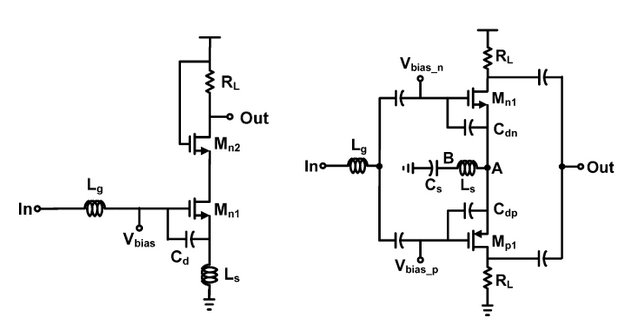
\includegraphics[width=0.5\textwidth]{figures/LNA.png}
    \caption{Cascode (left) and Current Reuse (right) structure, both figures borrowed from Cha et. al~\cite{lna}.}
    \label{fig:lna}
\end{figure}

It isn't clear exactly which structure would be better: cascode or current-reuse. As such, what follows is our analysis of current reuse to figure out if there are any problems with it.

With the current reuse structure, the active components are heavily restrained so as to limit the power consumption~\cite{lna}. As such, the passive networks depicted in Fig.~\ref{fig:lna} perform much of the gain~\cite{lna}. The power consumption is minimized by using this kind of structure since we need a small operating current to activate the MOSFETs and we will achieve gain from the other components. Additionally, the two transistors in the current reuse structure can be biased into subthreshold region to minimize the power consumption. The $g_m$ parameter of this component is the $g_m$ of NMOS plus the $g_m$ of the PMOS. In this way, the effective transconductance is larger than it would be otherwise. The gain of the current reuse LNA is:

\begin{equation} 
  	A_{v} = \frac{g_{mtot}}{2R_s \omega_0 C_{gs}}Z_{load}
	\label{eq:lnagain}
\end{equation}

The $C_{gs}$ given in (\ref{eq:lnagain}) is the total $C_{gs}$ of the stacked transistor pair.  The input matching should be matched to 50 $\Omega$. From the gates of the transistors, the input impedance would be given by:

\begin{equation} 
  	Z_{in}(j\omega)=\frac{g_mL_s}{C_{gs}} + j[\omega (L_s+L_g) - \frac{1}{\omega C_{gs}}]
	\label{eq:inputimp}
\end{equation}

The real part in (\ref{eq:inputimp}) should be matched to 50 $\Omega$, and imaginary part should be matched to 0 $\Omega$. Input matching is a simple problem. Output matching, however, is much more difficulty. Examining the output impedance:

\begin{equation} 
  	Z_{out}(j\omega) = r_0 + j\omega\frac{(r_0g_{mtot}L_s+L_s-\omega^2L_sL_gC_{gs})}{1-(L_s+L_g)C_{gs}\omega^2}
\end{equation}

The imaginary part has the same two poles, but also the pole which is considered to be the center frequency. At the center frequency, the imaginary part diverges to infinity -- this makes it difficult to do the output matching. Because of this reason, we switched back to the cascode structure is used.

In the cascode structure, the common source amplifier is the main amplifier. By applying the common gate, we can get good reverse isolation since there is no connecting path for current to flow between the ports when the gate is an AC ground ~\cite{Razavi}. Fortunately, the input impedance of this structure is the same as the current reuse one (\ref{eq:inputimp}). Thus, the input matching can be easily achieved. The output impedance of the cascode structure is given by:

\begin{equation} 
  	Z_{out}(j\omega) = \frac{SLR_L}{j\omega L+R_L-\omega^2LCR_L}
\end{equation}

At the center frequency, the output impedance can be made equal to  the load resistance of the next stage. Next, we consider the gain parameters of this structure. The gain is given by:

\begin{equation} 
  	A_{v} = \frac{R_L}{2\omega_0L_s}
\end{equation}

The load resistor and center frequency are fixed parameters. To get a high gain with this LNA, the only free parameter that can be adjusted is the source degenerated inductor. However, this inductor is selected in such a way as to perform input matching. This is where the iterative design process begins to take off and now all the components can be carefully selected to get good results.

\subsection{Mixer}

A mixer takes two signals and produces an output that contains both the sum and the difference of the frequencies of the original signals. Mixers can be subclassed into active mixers and passive mixers. For our purposes, we need the mixer stage to exhibit some gain to meet design criteria so passive mixers were never considered. 

Internally, active mixers split down into single balanced and double balanced mixers. Double-balanced mixers can provide better input linearity, relatively low noise, and completely isolate the LO to RF ports resulting in very little feedthrough when compared to single balanced mixers. The cons are that the circuit requires large off-chip baluns/transformers to split the signal outputs if the other components do not do it already. 

\subsubsection{Design Procedure}
The typical mixer implementation is a standard Gilbert cell~\cite{gilbert}, which is a stock double-balanced mixer. The Gilbert cell original design doesn't have low noise, consumes relatively high power (for MedRadio), and needs to operate from a much larger supply voltage (must be capable of activating all transistors across ground). We employed the modified Gilbert cell from Krcmar et. al~\cite{krcmar1}. It is pictured in Fig.~\ref{fig:mixer}. 

\begin{figure}[h]
   \centering
    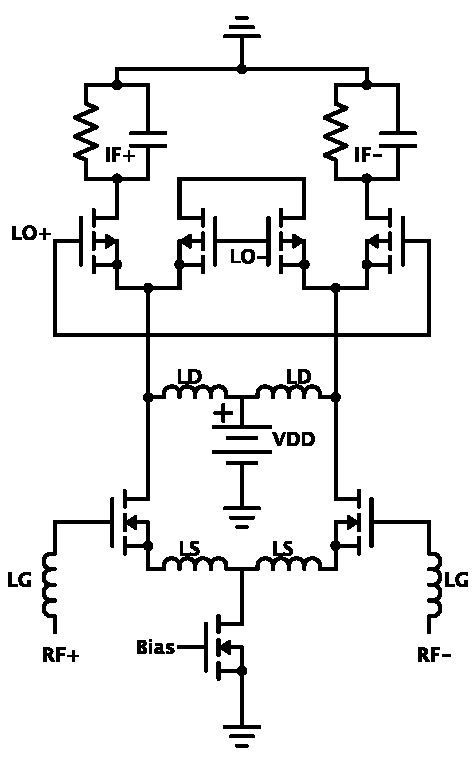
\includegraphics[width=0.40\textwidth]{figures/Mixer.pdf}
    \caption{
        Circuit schematic of the modified Gilbert cell~\cite{krcmar1} used in our mixer. The top row of PMOS transistors are the switching pairs. The middle row of NMOS transistors are the transconductors with current being driven by the current sink at the bottom.
    }
    \label{fig:mixer}
\end{figure}

The advantages of this circuit is that the biasing of the switching pairs and the transconductors are now totally separated, allowing it to operate at a lower supply voltage without weakening circuit operation\~cite{krcmar1}. The transconductors have control over the gain portion of the circuit and need to have careful current control through them, hence a current sink is connected to the source of the MOSFETs. For the switching pairs, the PMOS are biased to be barely on; mostly off.  The VCO signal will come into the switching pairs and quickly switch it into saturation and then back out again. It is to our disadvantage if the switching pairs enter the triode region since that will reduce the linearity and cause the gain to compress faster~\cite{Razavi}. 

The source and gate inductors connected to the transconductors are selected for input matching and to resonate the circuit. The drain inductor is sized to resonate with the VCO's parasitic source capacitance~\cite{krcmar1}. Accordingly, the input impedance is given by:

\begin{equation} 
  	Z_{in}(j\omega) = \frac{g_{m}}{C_{gs}}L_{source}+j(\omega[L_{source}+L_{gate}]-\frac{1}{\omega C_{gs}})
	\label{eq:mixerZin}
\end{equation}

The resonance frequency is given by:

\begin{equation}
\omega = \frac{1}{\sqrt{C_{gs}(L_{source}+L_{gate})}}
\end{equation}

The source inductor is selected to match to an input resistance:

\begin{equation}
L_{source} = \frac{R_{input}}{\frac{g_{m}}{C_{gs}}}
\end{equation}

While the gate inductor is selected to achieve resonance at the input frequency to the transconductors:

\begin{equation}
L_{gate}=\frac{1-\omega^{2}L_{source}C_{gs}}{\omega^{2}C_{gs}}
\end{equation}

With these equations, the values of the gate and drain inductors can be properly chosen.
The conversion gain of the double balanced mixer is given typically by~\cite{Razavi}:

\begin{equation}
C.G. = \frac{2}{\pi}g_{m}Z_{out}
\end{equation}

Because of the input matching the transconductance term is modified and the final equation becomes:
\begin{equation}
C.G. = \frac{1}{\pi}\frac{g_{m}Z_{out}}{\sqrt{(1-\omega^{2}L_{source}C_{gs})^{2}+(\omega L_{source}g_{m})^{2}}}
\end{equation}

As a starting point, we made an assumption for the value of $C_{gs}$ using estimates culled from the IBM7RF~\cite{ibm7rf} library for the NMOS transistors and also assumed the output impedance was a single load resistor matched to 50 $\Omega$. Using that, we were able to make substitutions into the C.G. equation and solved for the desired value of the transconductance. After that, the input inductors were sized using the previous equations and assuming a center frequency of 403.5 MHz. Our initial design estimate assumed the current to start at 1 mA and we were able to get the sizing ratio using the below:

\begin{equation}
\frac{W}{L} = \frac{g_{m}^2}{2K_{n}I}
\end{equation}

Finally, the drain inductor values were obtained assuming simple resonance:

\begin{equation}
L_{drain} = \frac{1}{\sqrt{\omega^{2}_{VCO}C_{gs}}}
\end{equation}

At this point, the circuit was fully sized and allowed us to begin iterating the design to achieve the desired results.
The parameters that affected our results the most are as follows:

\begin{itemize}
	\item Width. This affected virtually every figure of merit (noise, gain, linearity), so it had to be tuned with great care. Accordingly, we wanted to keep the width below the millimeter scale at all costs.
	\item Switching DC bias and VCO swing. The DC bias of the LO PFETs was selected at a point where the VCO would have to swing as little as possible to switch the transistor from off to saturation (in order to reduce VCO power consumption). This primarily affected the gain and linearity of the circuit.
	\item Transistor fingers. The more fingers available lowered the parasitics of the transconductor stages. Increasing the fingers led to improved noise figure and linearity.
	\item Input impedance. The value of the input impedance had a large effect on our noise figure; we opted to increase the value we input matched to in order to reduce our overall noise.
	\item Output impedance. We needed to increase the gain without increasing the current. The only way to do that was to increase the size of the load resistor.
	\item Inductor values. The inductor values needed to be swept to compensate for tradeoffs between linearity and gain. The source inductor was kept relatively constant but the gate and drain inductors were tweaked often in an effort to improve the linearity of the mixer.
\end{itemize}

These are a small subset of the variables used when iterating over the design. Results are discussed later on.

\subsection{Voltage Controlled Oscillator}
As shown in Figure \ref{fig:vco}, the proposed single-ended VCO uses a pair of complementary PN-MOSFETs so that the DC current can be reused and a low power VCO can be realized, following the logic given by Jang et. al~\cite{vco}. The LC tank determines the oscillation frequency:

\begin{equation}
\omega_{0} = \frac{1}{\sqrt{L_2C_V}}
\end{equation}

Note that, $C_V$ includes the varactors as well as the parasitic gate-source and drain-source capacitors of the PN-MOSFETs. The varactors are used to tune the VCO oscillation frequency and the transistors are configured to provide a negative resistance to compensate for the tank loss. 

\begin{figure}[h]
   \centering
    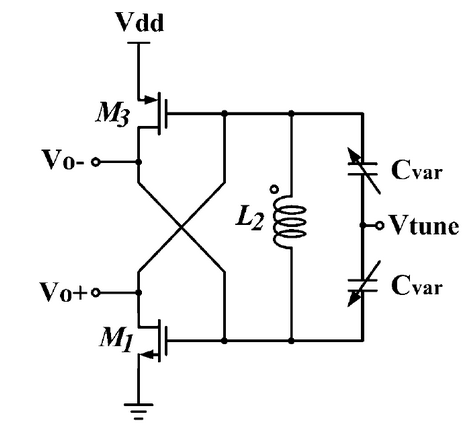
\includegraphics[width=0.50\textwidth]{figures/VCO.png}
    \caption{Schematic of the VCO, borrowed from Jang~\cite{vco}.}
    \label{fig:vco}
\end{figure}


The NMOS has the dimension of $\frac{W}{L}=\frac{30}{0.18}$ and the PMOS has the dimension of $\frac{W}{L}=\frac{200}{0.18}$, both in micro. The values for inductor and varactors are optimized to center the oscillation frequency at 400 MHz.

